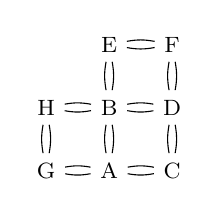
\begin{tikzpicture}[scale=0.8]
    % \tikzstyle{v}=[draw, circle, minimum size=0.1cm, scale=0.7, font=\footnotesize]
    \tikzstyle{v}=[font=\footnotesize]

    \node[v] (a) at (0,0) {A};
    \node[v] (b) at (0,1) {B};
    \node[v] (c) at (1,0) {C};
    \node[v] (d) at (1,1) {D};
    \node[v] (e) at (0,2) {E};
    \node[v] (f) at (1,2) {F};
    \node[v] (g) at (-1,0) {G};
    \node[v] (h) at (-1,1) {H};

    \draw (a) to [bend right=10](b);
    \draw (a) to [bend left=10](b);
    \draw (a) to [bend right=10](c);
    \draw (a) to [bend left=10](c);
    \draw (d) to [bend right=10](c);
    \draw (d) to [bend left=10](c);
    \draw (b) to [bend right=10](d);
    \draw (b) to [bend left=10](d);
    \draw (b) to [bend right=10](e);
    \draw (b) to [bend left=10](e);
    \draw (b) to [bend right=10](h);
    \draw (b) to [bend left=10](h);
    \draw (g) to [bend right=10](h);
    \draw (g) to [bend left=10](h);
    \draw (g) to [bend right=10](a);
    \draw (g) to [bend left=10](a);
    \draw (f) to [bend right=10](e);
    \draw (f) to [bend left=10](e);
    \draw (f) to [bend right=10](d);
    \draw (f) to [bend left=10](d);
\end{tikzpicture}